\begin{figure*}[!htb]
	\centering
	\begin{subfigure}{1.0\textwidth}
		\centering
		\caption{}
		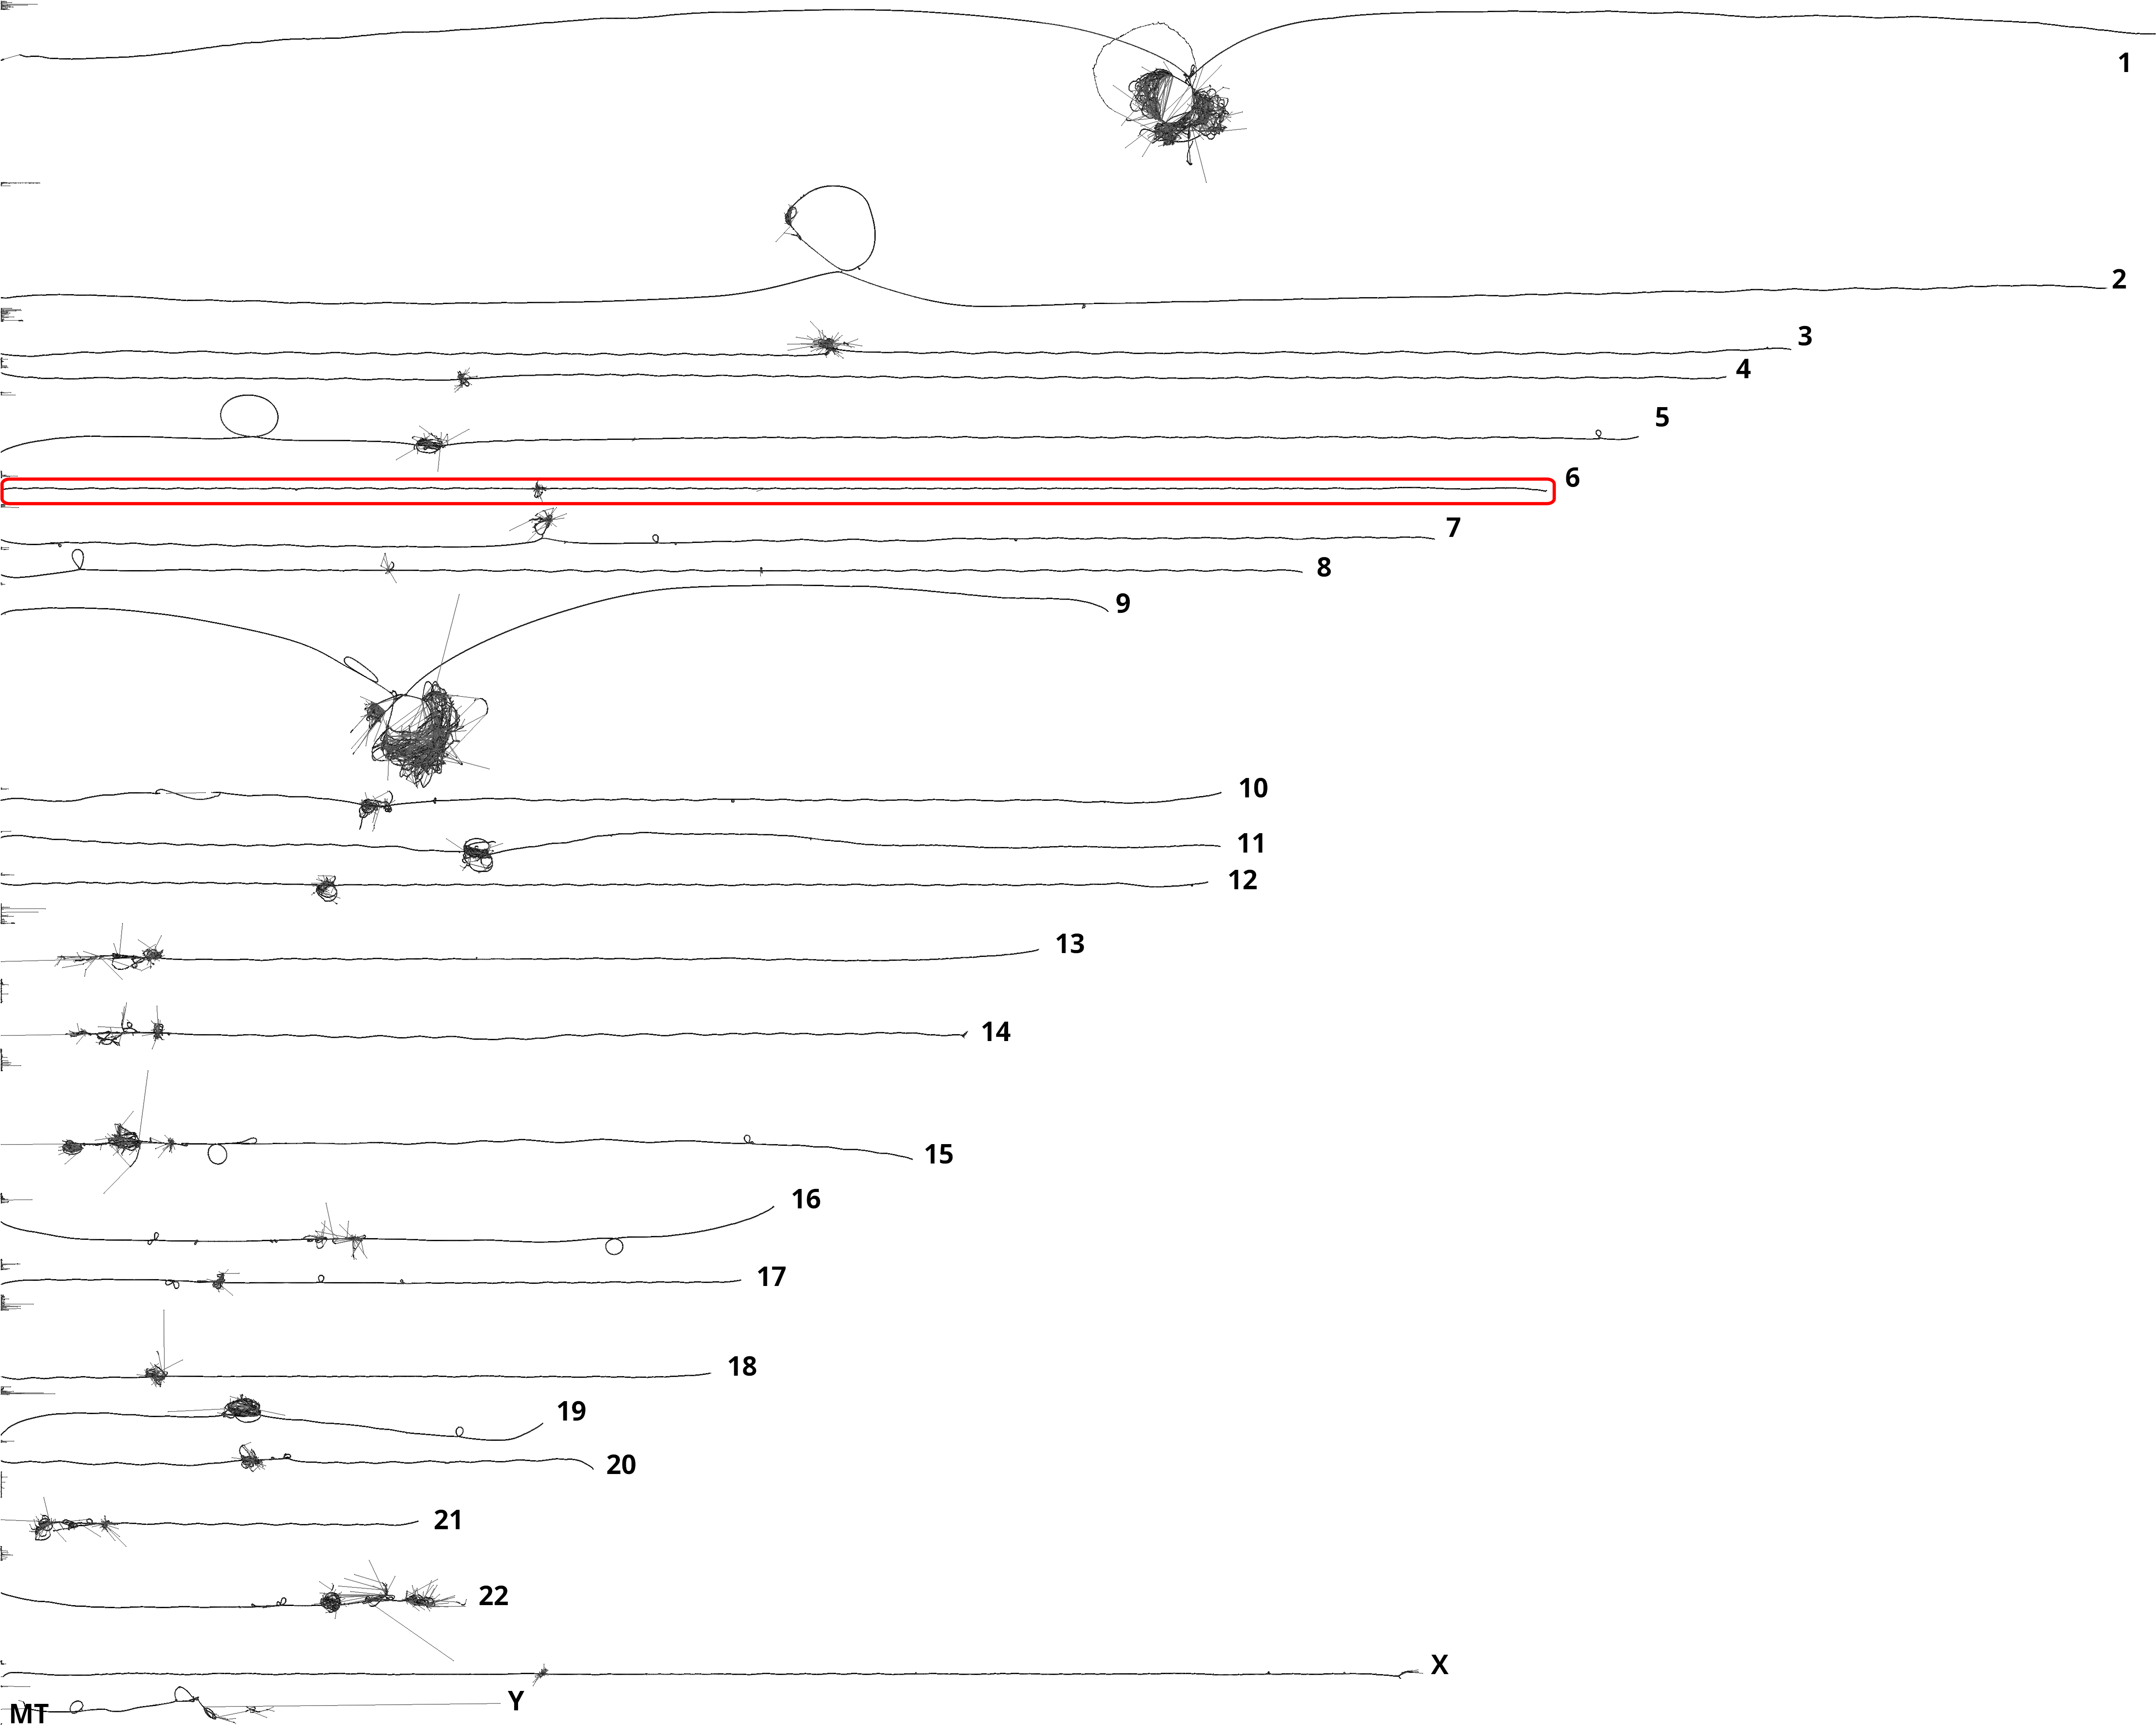
\includegraphics[width=1.0\linewidth]{fig/2D/hprc-v1.0-pggb.og.lay.H4000.r4.0-highlighted.png}
		\label{fig:sfig1}
	\end{subfigure}
	\\
	\begin{subfigure}{1.0\textwidth}
		\centering
		\caption{}
		
\includegraphics[width=1.0\linewidth]{fig/2D/grch38.chr6.MHC_annotated.png}
		\label{fig:sfig2}
	\end{subfigure}
	\\
	\begin{subfigure}{1.0\textwidth}
		\centering
		\caption{}
		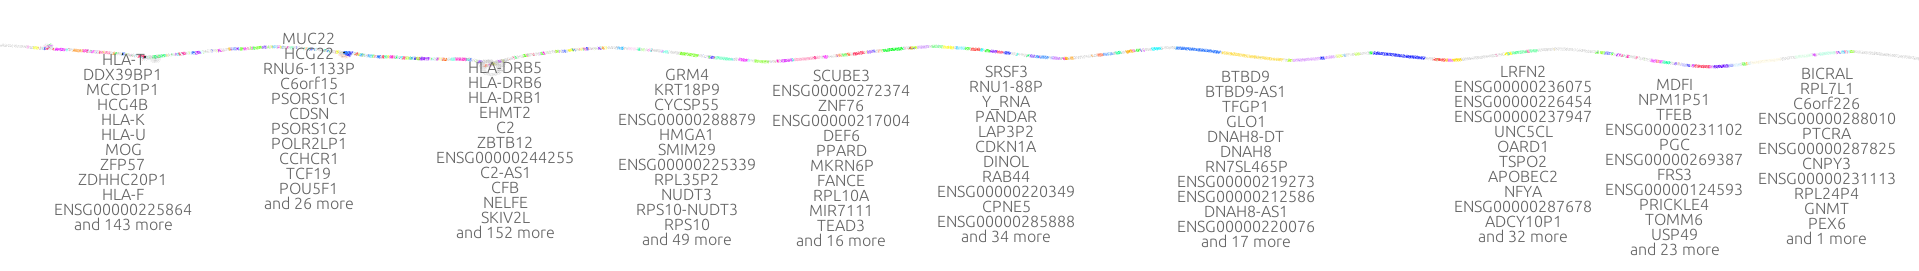
\includegraphics[width=1.0\linewidth]{fig/2D/grch38.chr6.MHC_genes_annotated.png}
		\label{fig:sfig3}
	\end{subfigure}
	\\
	\begin{subfigure}{1.0\textwidth}
		\centering
		\caption{}
		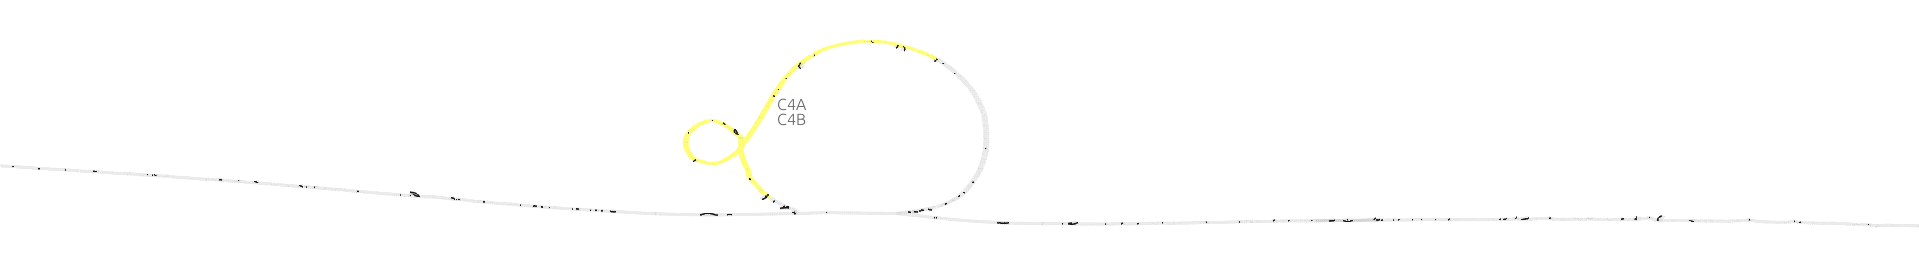
\includegraphics[width=1.0\linewidth]{fig/2D/grch38.chr6.C4_gene_annotated.png}
		\label{fig:sfig4}
	\end{subfigure}	
	\caption{2D visualizations of all chromosomes of the Human Pangenome Resource Consortium (HPRC) 90 haplotypes pangenome graph, chromosome 6, the major histocompatibility complex (MHC), and the complement component 4 (C4). 
		\textbf{(a)} \textit{odgi draw} layout of the HPRC pangenome graph 90 haplotypes. 
		Displayed are all 24 autosomes and the mitochondrial chromosome.
		A red rectangle highlights chromosome 6 which is shown in the subfigure below. 
		\textbf{(b)} \textit{gfaestus} screenshot of the chromosome 6 layout. 
		Colored in blue is the MHC. 
		The hairball in the middle is the centromere. 
		The black structures in the centromere are edges. 
		\textbf{(c)} \textit{gfaestus} screenshot of the MHC. 
		All MHC genes are color annotated and the names of the genes appear as a text overlay. 
		\textbf{(d)} \textit{gfaestus} screenshot of the region around C4, specifically color highlighting genes C4A and C4B. 
		The black lines are the edges of the graph.}
	\label{fig:2d_layouts}
\end{figure*}